  
%% \listfiles
\documentclass[apj]{emulateapj}
%\documentclass[preprint2,12pt]{emulateapj}
%% \usepackage{natbib}
\usepackage{graphicx}
\usepackage{epsfig}
\usepackage{amssymb,amsmath}
\usepackage{array}
\usepackage{threeparttable}
\usepackage{hyperref,graphicx}    

\doublespace

%definitions
\newcommand{\Msol}{${\rm M_{\sun}}$}


%% Editing markup...
\usepackage{color}


%%%%%%%%%%%%%%%%%%%%%%%%%%%%%%%%%%%%%%%%%%%%%%%%%%%%%%%%%%%%%%%%%%%%%%%%%%%
% WARNING: This LaTeX block was generated automatically by authors.py
% Do not change by hand: your changes will be lost.

%%%%%%%%%%%%%%%%%%%%%%%%%%%%%%%%%%%%%%%%%%%%%%%%%%%%%%%%%%%%%%%%%%%%%%%%%%%


% --------------------- Ancillary information ---------------------
\shortauthors{SURP et al.}
\shorttitle{CITA Final Project}




\begin{document}

\title{CITA Final Project: Introduction to Galpy}
 %% ---------
 
\author{Yumna Arshad}
%\altaffiltext{1}{CITA, University of Toronto}
 
\section{Introduction}
My final project aims to introduce the methods of galpy, a module in python used for modelling the orbital dynamics of objects in the galaxy. 
The project consists of 2 parts. 
The first part is an introductory approach to galpy and focuses on specifically learning how to use both potential and orbit objects from the module as well as the various methods associated with them.
The second part consists of modelling the accretion of a globular cluster, that is initially bound to a satellite galaxy of the Milky Way, onto the Milky Way galaxy itself. 


\section{Part 1: Intro to Galpy Methods}

For this part of the project there are 3 separate tasks: 1) plotting rotation curve of MW galaxy, 2) integrating orbit of Sun and 3) integrating orbit of a specific tidal stream named GD -1.


\subsection{Rotation Curve of MW Galaxy}
To plot the rotation curve of the MW galaxy I created 3 different potential instances corresponding to the potential of the disk, bulge and halo separately and plotted them on one plot using the plotRotcurve method. Then I summed up all the potentials to create the overall galactic rotation curve which peaks at around 225 km/s and slowly declines afterward, this is the sum of the bulge, disk and halo potentials.
A plot of these rotation curves can be seen in Fig.\ref{fig:Q1_rot_curve}.


\begin{figure}
    \centering
    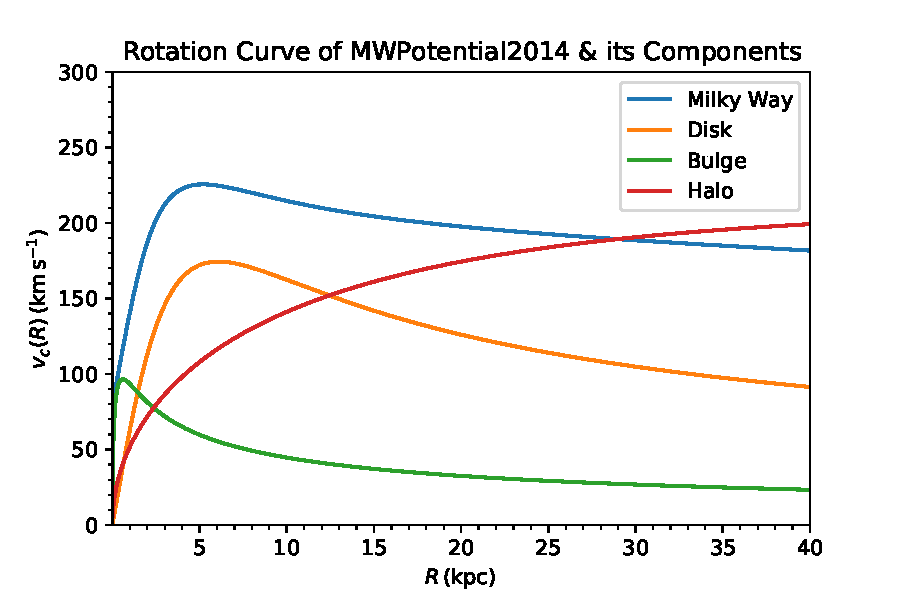
\includegraphics[width=1.0\columnwidth]{Q1a.pdf}
    \caption{Plot of the rotation curve of the Milky Way Galaxy including its labelled components: bulge, halo and disk.}
    \label{fig:Q1_rot_curve}
\end{figure}

\subsection{Orbit of Sun in MW Galaxy}
To plot the orbit of the Sun in the MW Galaxy I initialized an Orbit instance and integrated it for 10 Gyr using the MW potential in part 1 to properly model the orbit.
I used the plot method of the sun orbit object to display the plot. 
A figure of this plot is shown in Fig.\ref{fig:Q1_Sun}


\begin{figure}
    \centering
    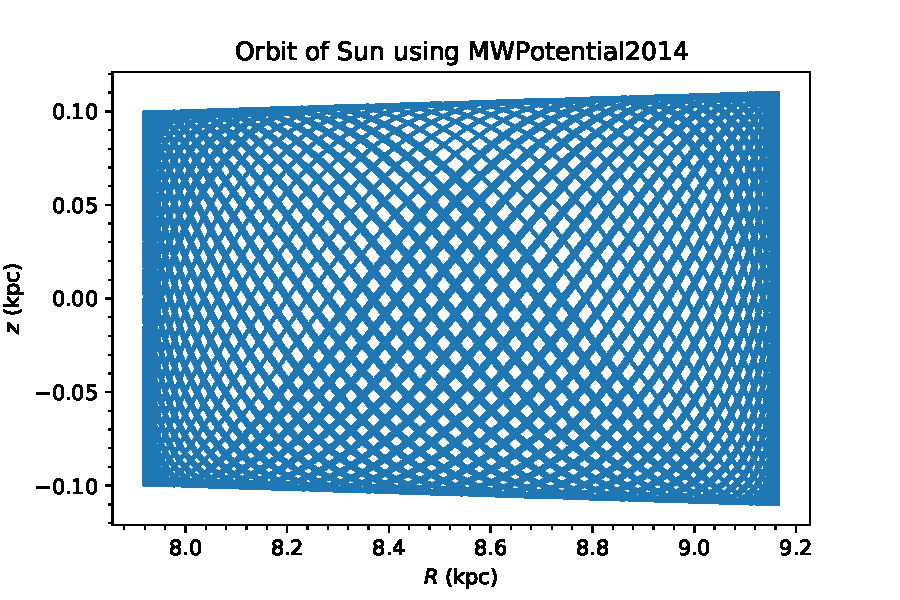
\includegraphics[width=1.0\columnwidth]{Q1b.pdf}
    \caption{Plot of the orbit of the Sun in Milky Way potential for 10 Gyr (integrated forward). The orbit is plotted as: vertical height above plane of galaxy in kpc as a function of galactocentric radius in kpc.}
    \label{fig:Q1_Sun}
\end{figure}



\subsection{GD-1 Tidal Stream}
The path of GD-1 tidal stream in the sky is plotted by: initializing an orbit object with the given coordinates for the stream as specified in paper by Bovy and Webb \cite{GD-1}.
Figures showing the GD-1 stream in declination vs right ascension are shown in Fig.\ref{fig:Q1_radec_f} (integrated forwards) and in Fig.\ref{fig:Q1_radec_b} (integrated backwards).
Figures showing the GD-1 stream in distance (from the Sun) vs right ascension are shown in Fig.\ref{fig:Q1_radist_f} (integrated forwards) and in Fig.\ref{fig:Q1_radist_b} (integrated backwards).
For all 4 orbits, the integration period is 50 Myr either forwards or backwards in time.

\begin{figure}
    \centering
    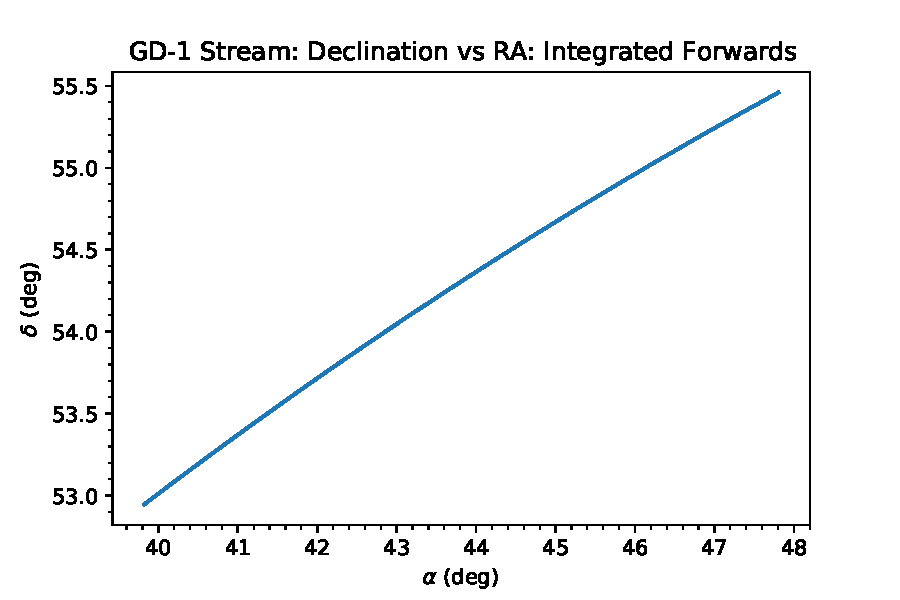
\includegraphics[width=1.0\columnwidth]{Q1c_1.pdf}
    \caption{Tidal stream GD-1's declination vs right ascension integrated forwards in time.}
    \label{fig:Q1_radec_f}
\end{figure}

\begin{figure}
    \centering
    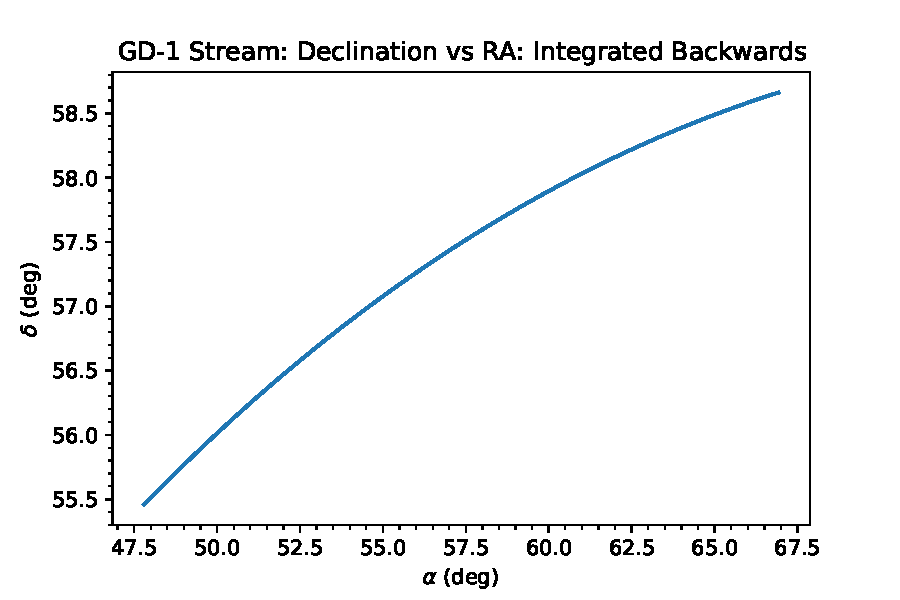
\includegraphics[width=1.0\columnwidth]{Q1c_3.pdf}
    \caption{Tidal stream GD-1's declination vs right ascension integrated backwards in time.}
    \label{fig:Q1_radec_b}
\end{figure}

\begin{figure}
    \centering
    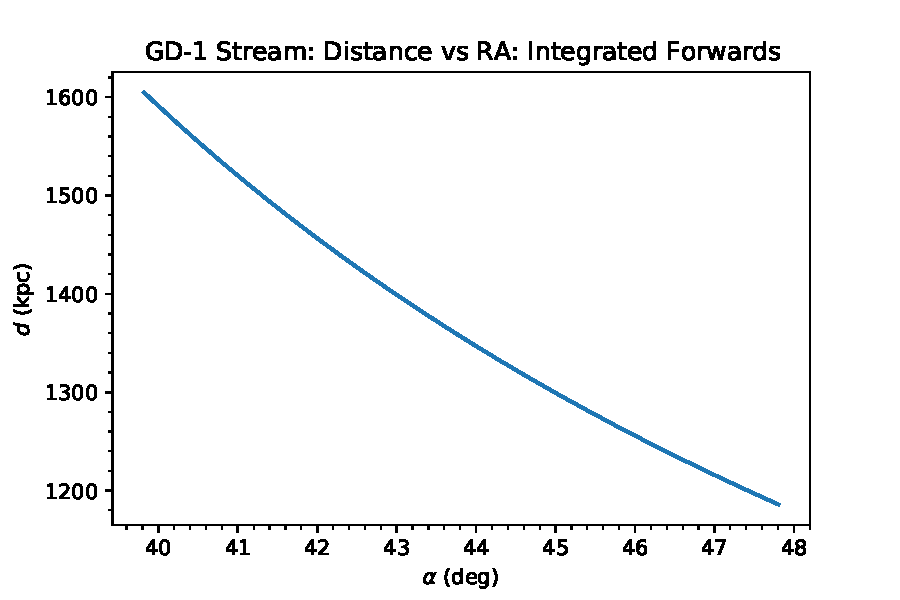
\includegraphics[width=1.0\columnwidth]{Q1c_2.pdf}
    \caption{Tidal stream GD-1's distance (from Sun) vs right ascension integrated forwards in time.}
    \label{fig:Q1_radist_f}
\end{figure}

\begin{figure}
    \centering
    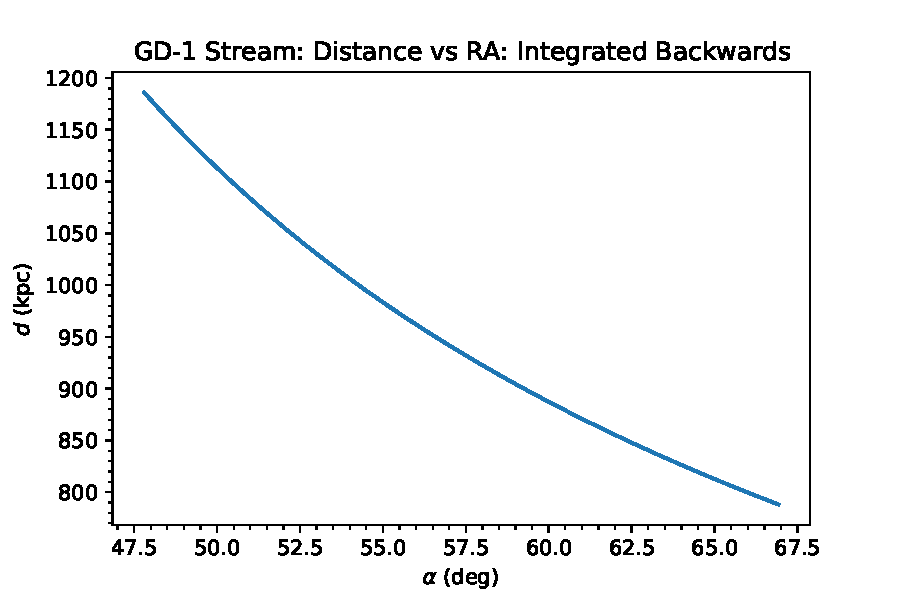
\includegraphics[width=1.0\columnwidth]{Q1c_4.pdf}
    \caption{Tidal stream GD-1's distance (from Sun) vs right ascension integrated backwards in time.}
    \label{fig:Q1_radist_b}
\end{figure}


\section{Part 2: Stimulating Accretion of Globular Cluster onto Milky Way}

\subsection{Method}
To stimulate the accretion of a globular cluster onto the Milky Way Galaxy: the first thing I did was import and integrate the orbits of all the satellite galaxies of the Milky Way and plotted their apocenters and pericenters vs their current galactocentric radii. 
Using these plots, the satellite with the smallest pericenter is identified to be TucanaIII and the time at which it 1st reaches its smallest galactocentric radius is -1.77 Gyr (i.e 1.77 Gyr in the past). This satellite will be used to model the accretion of the globular cluster. 
To begin with, the orbit of TucanaIII integrated backwards for 10 Gyr is plotted with the effects of dynamical friction included. Dynamical friction is implemented using an instance of the ChandrasekharDynamicalFrictionForce with the density of the MW potential (imported using MWPotential2014 which is a list of potential objects making up the Milky Way) and given satellite parameters such as mass and size. Then, the orbit of the satellite is integrated back in time using the combined potential of the MW and the dynamical friction. This orbit is shown in Fig.\ref{fig:Q2_cdf}. The radius of the satellite at 10 Gyr is determined to be 240.6 kpc.
\begin{figure}
    \centering
    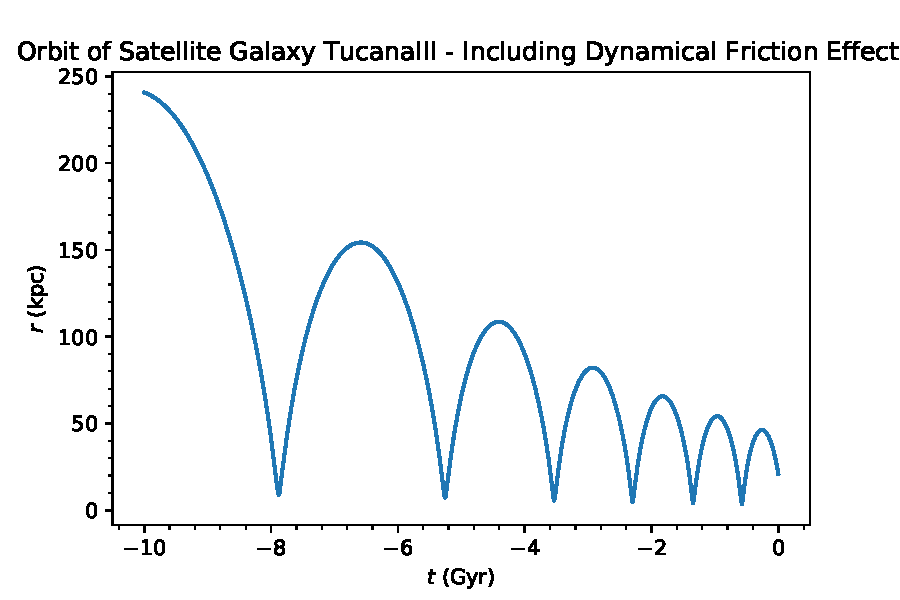
\includegraphics[width=1.0\columnwidth]{Q2c.pdf}
    \caption{Plot showing the orbit of TucanaIII satellite galaxy, the satellite with the smallest pericenter radius, integrated backwards in time for 10 Gyr. The orbit is shown in radius vs time.}
    \label{fig:Q2_cdf}
\end{figure}

A star-cluster is then initialized to be on a circular orbit of radius 4 kpc within the satellite galaxy, the orbital velocity can be determined using Eq.\ref{equation: v_circ} and this gives a velocity of $\approx$ 328 km/s.

\begin{equation}
     v = \sqrt{\frac{GM}{r}}
    \label{equation: v_circ}
\end{equation}

As well, the satellite + cluster system are moved to the radius determined above (i.e. 240.6 kpc). To model the orbit of the satellite characerized by a Hernquist potential, a MovingObjectPotential object instance is created with the associated orbit being that of the satellite as previously determined, i.e. orbit of TucanaIII. 
Finally, the orbits of both the satellite and the star-cluster are integrated and plotted. The results are shown in Fig.\ref{fig:Q2_satellite} and Fig.\ref{fig:Q2_star_cluster}, respectively. 

\begin{figure}
    \centering
    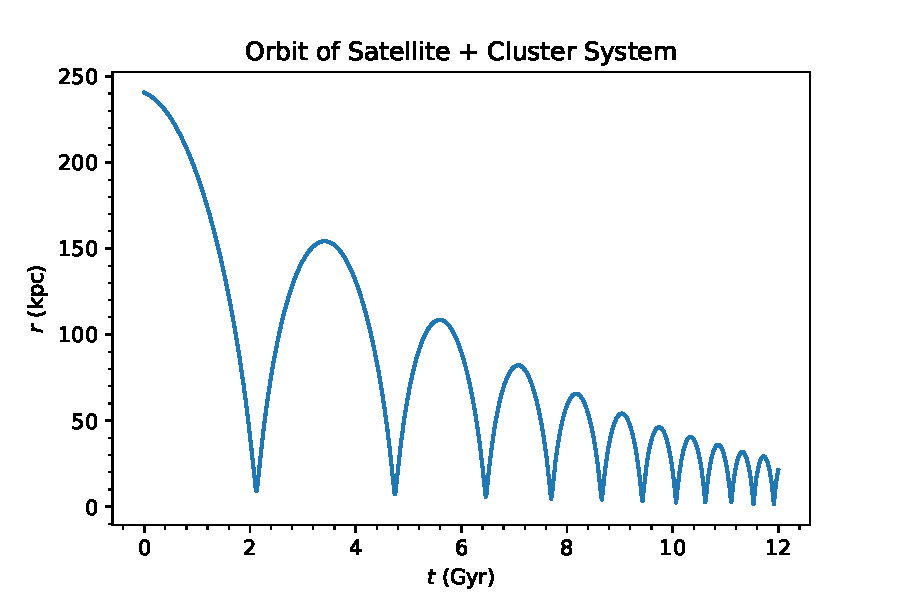
\includegraphics[width=1.0\columnwidth]{Q2_sat.pdf}
    \caption{Plot showing the orbit of the satellite galaxy integrated forwards in time for 12 Gyr. The orbit is shown in radius vs time and includes the effects of dynamical friction.}
    \label{fig:Q2_satellite}
\end{figure}

\begin{figure}
    \centering
    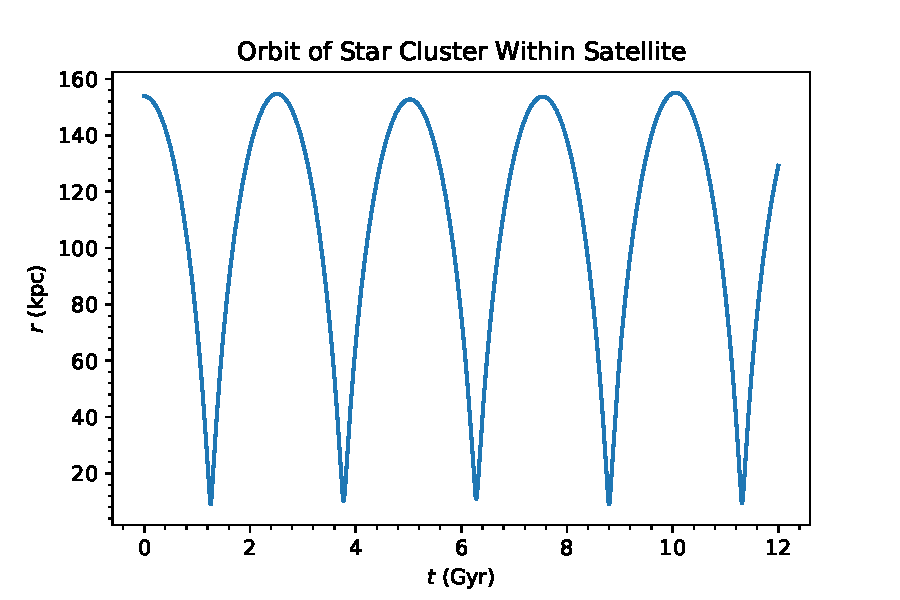
\includegraphics[width=1.0\columnwidth]{Q2_sc.pdf}
    \caption{Plot showing the orbit of the star-cluster system within the satellite galaxy for 12 Gyr. Note that r is the galactocentric distance, plotted as a function of time.}
    \label{fig:Q2_star_cluster}
\end{figure}




\subsection{Comment on Orbits of Star Cluster and Satellite Galaxy}
The orbit of the satellite galaxy as shown in Fig.\ref{fig:Q2_satellite} is the same as the orbit in Fig.\ref{fig:Q2_cdf} since it initially starts at its position at -10 Gyr and follows the same path forward in time as it did to go back.
The star cluster's orbit within the satellite follows a bound orbit such that it becomes accreted onto the Milky Way galaxy as the satellite spirals in and remains bound to the MW galaxy.


\begin{thebibliography}{99}

\bibitem{GD-1}
J. J. Webb and J. Bovy, “Searching for the GD-1 stream progenitor inGaiaDR2 with directN-body simulations,” Monthly Notices of the Royal Astronomical Society, vol. 485, no. 4, pp. 5929–5938, 2019.



\end{thebibliography}


\end{document}

